\documentclass[12pt, a4paper]{article}

% Pakiety podstawowe
\usepackage[utf8]{inputenc}
\usepackage[polish]{babel}
\usepackage[T1]{fontenc}
\usepackage{geometry}
\geometry{a4paper, margin=2.5cm}

% Grafika i linki
\usepackage{graphicx}
\usepackage{float}
\usepackage{hyperref}
\usepackage{booktabs}
\usepackage{caption}

\usepackage{listings}
\usepackage{xcolor}

\definecolor{codegreen}{rgb}{0,0.6,0}
\definecolor{codegray}{rgb}{0.5,0.5,0.5}
\definecolor{codepurple}{rgb}{0.58,0,0.82}
\definecolor{backcolour}{rgb}{0.95,0.95,0.92}

\lstset{
    language=Python,
    backgroundcolor=\color{backcolour},   
    commentstyle=\color{codegreen},
    keywordstyle=\color{blue},
    numberstyle=\tiny\color{codegray},
    stringstyle=\color{codepurple},
    basicstyle=\ttfamily\footnotesize,
    breakatwhitespace=false,         
    breaklines=true,                 
    captionpos=b,                    
    keepspaces=true,                 
    numbers=left,                    
    numbersep=5pt,                  
    showspaces=false,                
    showstringspaces=false,
    showtabs=false,                  
    tabsize=4
}

\title{Dostrajanie predykcji opartej fuzzy logic z użyciem wybranej metaheurystyki inspirowanej naturą}
\author{Radosław Iskra, Rafał Oszajca, Artur Zamorowski}
\date{\today}

\begin{document}

\maketitle
\tableofcontents
\newpage

\section{Wstęp}
Podczas projektu użyto algorytmu inteligencji rojowej \textbf{GOA} (\textit{Grasshopper Optimization Algorithm}) \\ 
w celu dobrania parametrów dla układu Logiki Rozmytej (\textit{Fuzzy Logic}) służącego do 
wnioskowania ilości rozbłysków słonecznych klasy C w danym obszarze aktywnym na Słońcu. 
Układ wykorzystuje w tym celu dane o rozwoju plamy słonecznej, oraz jej aktywności z poprzednich 24 godzin.

\subsection{Model Hybrydowy}
Dobranie paramtrów modelu Logiki Rozmytej wymaga od projektanta szczegółowej wiedzy z rozważanego tematu.
Aby uniknąć zbędnego polegania na ręcznej regulacji parametrów, które jest nieefektywne i podatne na błędy, można
zastosować w tym celu algorytm metaheurystyczny, taki jak zastosowane przez nas GOA.

\subsection{System wnioskowania Rozmytego}
Projekt bazuje na systemie wnioskowania rozmytego typu Mamdani, zbudowanym od podstaw. Główne założenia teoretyczne tej części to:
\begin{itemize}
\item \textbf{Trójkątne funkcje przynależności:} Zmienne lingwistyczne (wejściowe np. rozwój plamy słonecznej, 
    wyjściowe np. klasa rozbłysku) są modelowane za pomocą trójkątnych funkcji przynależności 
    zdefiniowanych przez trzy punkty: \textit{a},\textit{b},\textit{c}.
\item \textbf{Generowanie reguł} Zamiast wpisywać reguły ręcznie, system wykorzystuje heurystykę i iloczyn kartezjański, aby pokryć wszystkie możliwe kombinacje wejść. Algorytm wylicza wynik dla danej kombinacji wejść i na jego podstawie dobiera odpowiedni zbiór wyjściowy.
\item \textbf{Wnioskowanie} Ewaluacja reguł opiera się na klasycznych operatorach rozmytych: minimum dla koniunkcji (AND) oraz maksimum dla alternatywy (OR). Defuzyfikacja (wyostrzanie) realizowana jest za pomocą metody środka ciężkości, co pozwala na uzyskanie ciągłej wartości liczbowej na wyjściu.
\end{itemize}

\subsection{Inteligencja Rojowa w Optymalizacji Parametrów}
Aby zminimalizować błąd predykcji (mierzony jako błąd średniokwadratowy - MSE), 
zaimplementowano Algorytm Optymalizacji Koników Polnych. Kluczowymi założeniami optymalizacji były:
\begin{itemize}
    \item \textbf{Funkcja Celu:} Algorytm ocenia jakość każdego osobnika (potencjalnego rozwiązania) mierząc wartość MSE między przewidywaniami systemu rozmytego a rzeczywistymi danymi treningowymi.
    \item \textbf{Redukcja Wymiarowości Przestrzeni Poszukiwań:} W teorii optymalizacji trzech zmiennych powinniśmy rozpatrywać 27 parametrów. W celu zredukowania skomplikowania niezbędnych optymalizacji, zdecydowano się na redukcję ilości wymiarów. 
        W tym celu "zablokowano" skrajne wartości funkcji brzegowych, a optymalizacji poddano jedynie wierzchołki funkcji trójkątnych. Umożliwiło to redukcję wymiarów do 3. Przyśpiesza to zbieganie algorytmu, i chroni przed utratą ciągłości logicznej systemu.
    \item \textbf{Eksploracja i Eksploatacja:} Współczynnik \textit{c} (zmniejszany liniowo z epoki na epokę) odpowiada za balansowanie między początkową szeroką eksploracją przestrzeni parametrów a końcową, bardziej precyzyjną, eksploatacją w okolicach najlepszego znalezionego rozwiązania globalnego.
\end{itemize} 

\section{Metodologia}
\subsection{Zbiór Danych i Preprocessing}
Do uczenia i testowania systemu wykorzystano publicznie dostępny zbiór danych \textbf{Solar Flare Data Set} z repozytorium UCI Machine Learning Repository. Zbiór ten zawiera kategoryczne i numeryczne cechy opisujące plamy słoneczne, a celem jest predykcja liczby rozbłysków słonecznych klasy C (zmienna ciągła).
Dane przygotowano do analizy poprzez:
\begin{itemize}
    \item Usunięcie braków danych
    \item Zakodowanie trzech pierwszych zmiennych kategorycznych na wartości liczbowe
    \item Podział na zbiór uczący (treningowy) i testowy w klasycznej proporcji 50/50, używając prostego podziału sekwencyjnego. 
\end{itemize}

\subsection{Definicja Przestrzeni i Zmiennych Lingwistycznych}
Ze względu na optymalizację czasu obliczeń autorskiego systemu rozmytego, do procesu wnioskowania wyselekcjonowano dwie kluczowe cechy wejściowe ze zbioru danych:
\begin{itemize}
    \item \texttt{evolution} (rozwój plamy słonecznej) - indeks 4.
    \item \texttt{prevActivity} (aktywność z poprzednich 24h) - indeks 5.
\end{itemize}

\subsection{Proces Optymalizacji}
W celu poprawy jakości predykcji, wyjściowe parametry funkcji przynależności poddano optymalizacji z wykorzystaniem algorytmu inteligencji rojowej Koników Polnych, przy poniższych założeniach:
\begin{itemize}
    \item \textbf{Rozmiar roju i epoki:} Populacja liczyła 100 osobników, a optymalizacja trwała 100 epok.
    \item \textbf{Redukcja wymiarowości:} Jak zostało opisane w poprzednich sekcjach, wymiarowość została zredukowana z 27 do 3. 
\end{itemize}

\newpage
\subsection{Kryteria Ewaluacji}
Aby obiektywnie ocenić zysk z zastosowania algorytmu rojowego, wygenerowane predykcje dla zbioru testowego oceniono za pomocą trzech standardowych metryk dla problemów regresji:
\begin{itemize}
    \item \textbf{Błąd średniokwadratowy (MSE)} - kładący duży nacisk na duże błędy.
    \item \textbf{Średni błąd bezwzględny (MAE)} - pokazujący średnią pomyłkę w oryginalnych jednostkach.
    \item \textbf{Współczynnik determinacji ($\mathbf{R^2}$)} - określający, jaką część wariancji zmiennej objaśnianej modeluje system.
\end{itemize}
Wyniki porównano dla trzech wariantów:
\begin{itemize}
    \item Autorski system rozmyty \textbf{przed optymalizacją} (z bazowym rozmieszczeniem funkcji).
    \item Autorski system rozmyty \textbf{po optymalizacji} (dostrojony przez algorytm GOA).
    \item System bazowy (baseline) wygenerowany z użyciem funkcji \texttt{pythonGenfis} z biblioteki \texttt{scikit-fuzzy}, która do predykcji wykorzystywała pełny zbiór 10 cech wejściowych.
\end{itemize}

\section{Wyniki Eksperymentów}

W tym rozdziale zaprezentowano obiektywne wyniki uzyskane podczas ewaluacji badanych modeli na wydzielonym zbiorze testowym. Zestawiono zarówno numeryczne metryki błędu, jak i wizualizacje przestrzeni decyzyjnych oraz funkcji przynależności przed i po zastosowaniu algorytmu GOA.

\subsection{Numeryczne wyniki ewaluacji}
Działanie trzech wariantów systemu oceniono za pomocą trzech metryk: błędu średniokwadratowego (MSE), średniego błędu bezwzględnego (MAE) oraz współczynnika determinacji ($R^2$). Zestawienie wyników znajduje się w Tabeli \ref{tab:wyniki_metryk}.

\begin{table}[H]
    \centering
    \caption{Zestawienie metryk ewaluacyjnych na zbiorze testowym}
    \label{tab:wyniki_metryk}
    \begin{tabular}{|l|c|c|c|}
        \hline
        \textbf{Model} & \textbf{MSE} & \textbf{MAE} & \textbf{$\mathbf{R^2}$} \\
        \hline
        System Autorski (Przed GOA) & 5.2253 & 1.7747 & -10.4042 \\
        System Autorski (Po GOA) & 6.4413 & 1.9242 & -13.0582 \\
        Skfuzzy (Model referencyjny) & 3.7645 & 1.7401 & -7.2161 \\
        \hline
    \end{tabular}
\end{table}

Na podstawie danych z Tabeli \ref{tab:wyniki_metryk} można zaobserwować, że najniższe wartości błędów (MSE i MAE) uzyskał model referencyjny Genfis. W przypadku systemu autorskiego, proces optymalizacji algorytmem rojowym GOA doprowadził do wzrostu błędów ewaluacyjnych na zbiorze testowym w stosunku do bazowej konfiguracji systemu.

\subsection{Porównanie funkcji przynależności}
Wykresy wygenerowane dla zmiennych wejściowych przedstawiają kształty trójkątnych funkcji przynależności. 
Wierzchołki dla modelu przed optymalizacją znajdowały się w punktach 1.0, 2.0 oraz 3.0. 
Wpływ algorytmu GOA na rozkład zarówno wykresu dla \textit{Evolution} jak i \textit{Previous Activity} jest wyraźnie widoczny.
W wyniku jego działania wierzchołki zostały przesunięte do [2.8, 2.8, 1.0] dla obu parametrów. 


\begin{figure}[H]
    \centering
    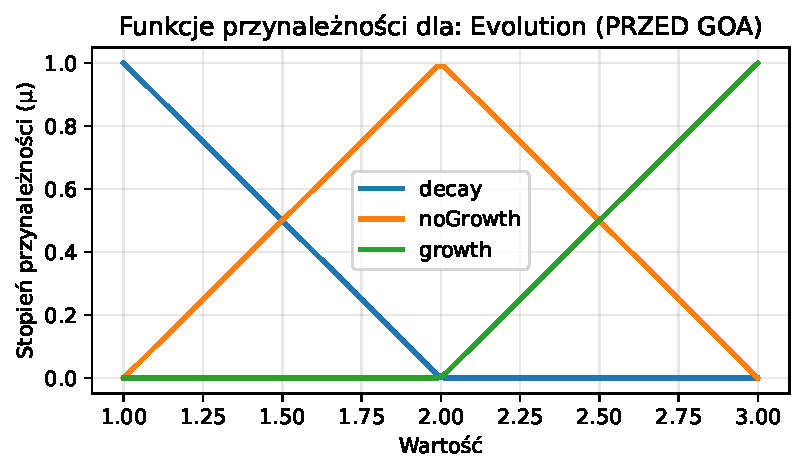
\includegraphics[width=0.45\textwidth]{../evo_preGOA.pdf}
    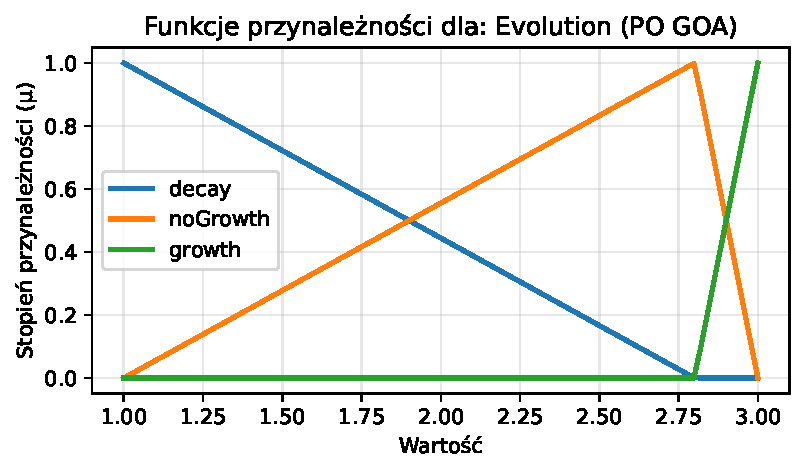
\includegraphics[width=0.45\textwidth]{../evo_postGOA.pdf}
    \caption{Porównanie wejściowych funkcji przynależności dla zmiennej \textit{Evolution} przed (lewa) i po (prawa) optymalizacji GOA.}
    \label{fig:mf_comparison}
\end{figure}

\begin{figure}[H]
    \centering
    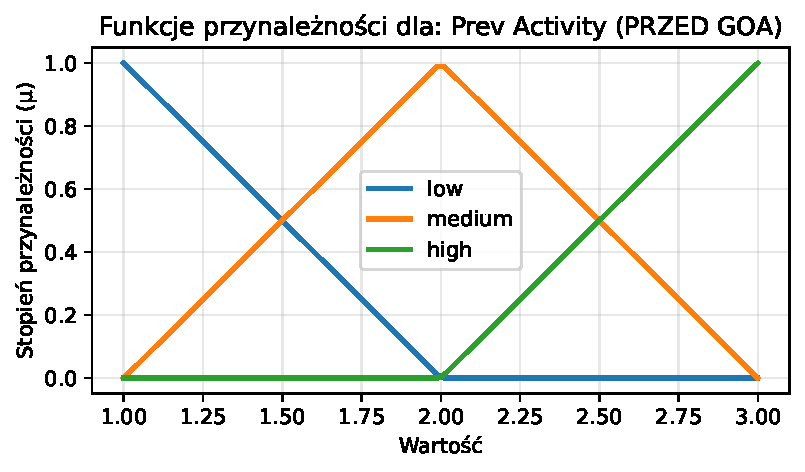
\includegraphics[width=0.45\textwidth]{../PrevActiv_preGOA.pdf}
    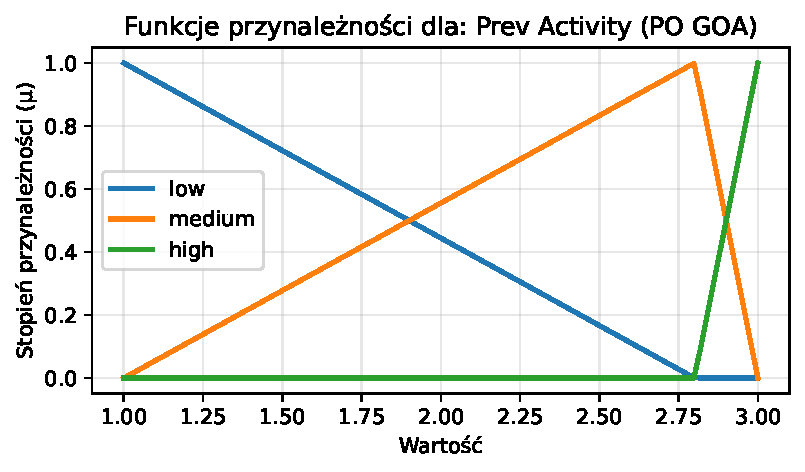
\includegraphics[width=0.45\textwidth]{../PrevActiv_postGOA.pdf}
    \caption{Porównanie wejściowych funkcji przynależności dla zmiennej \textit{Previous Activity} przed (lewa) i po (prawa) optymalizacji GOA.}
    \label{fig:mf2_comparison}
\end{figure}

\newpage
\subsection{Analiza powierzchni decyzyjnych}
Równie zauważalne zmiany między modelem bazowym a zoptymalizowanym uwidaczniają się na wykresach powierzchni decyzyjnych (tzw. heatmapach z interpolacją), 
które mapują przestrzeń dwóch zmiennych wejściowych na przewidywaną liczbę rozbłysków słonecznych.

\begin{figure}[H]
    \centering
    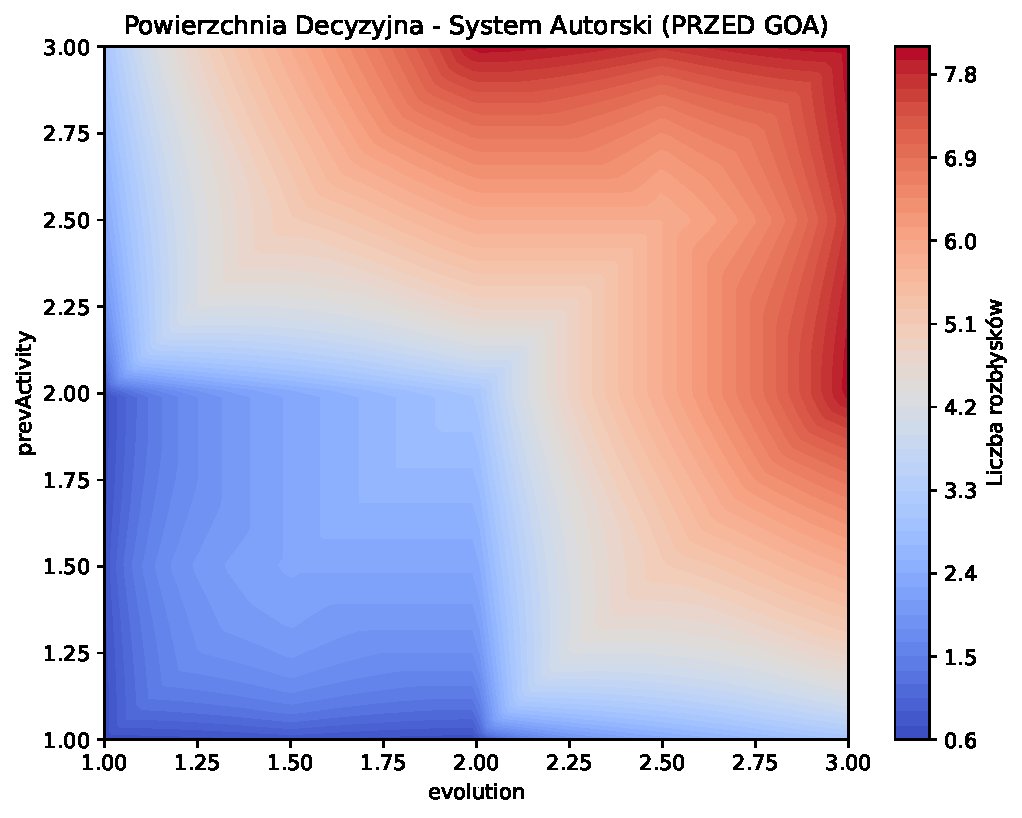
\includegraphics[width=0.45\textwidth]{../heatmap_preGOA.pdf}
    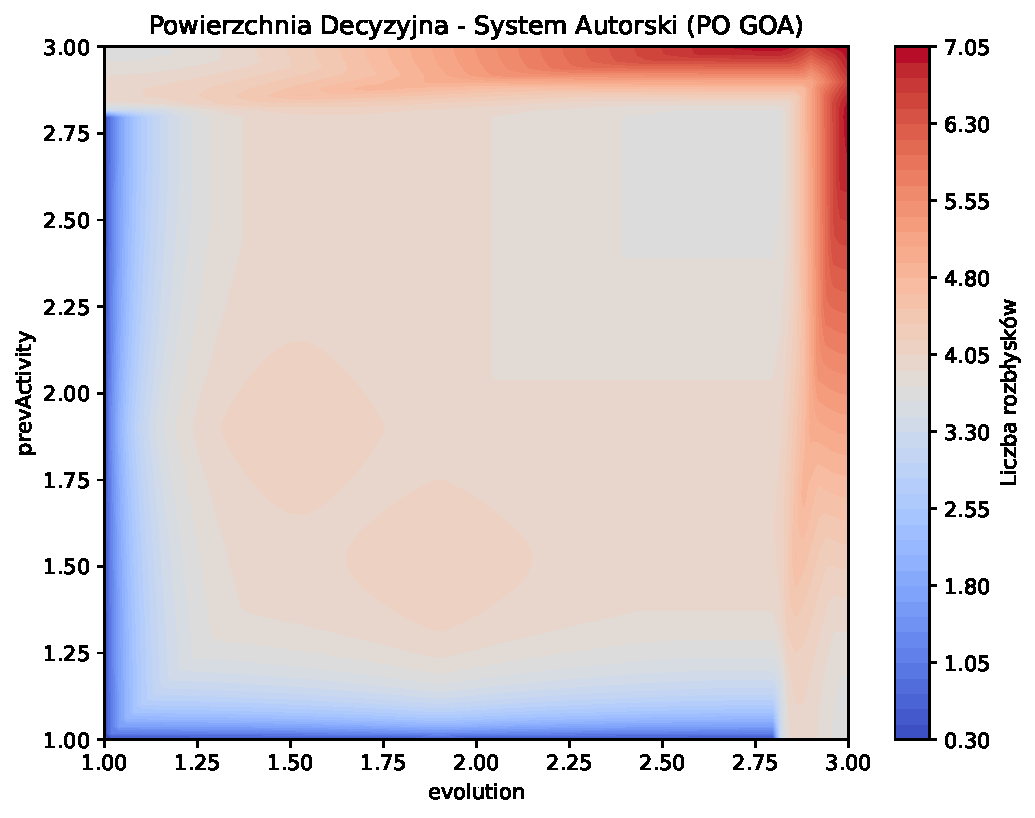
\includegraphics[width=0.45\textwidth]{../heatmap_postGOA.pdf}
    \caption{Powierzchnie decyzyjne systemu przed (lewa) oraz po (prawa) optymalizacji algorytmem GOA.}
    \label{fig:heatmaps}
\end{figure}

Powierzchnia decyzyjna systemu przed zastosowaniem algorytmu GOA (Rysunek \ref{fig:heatmaps}, lewa strona) charakteryzuje się płynnymi, 
geometrycznymi przejściami gradientowymi w całej przestrzeni. 
Najwyższe prognozowane wartości zlokalizowane są w prawym górnym rogu 
przestrzeni wejściowej, osiągając maksimum w okolicach wartości 7.8. 

Z kolei powierzchnia systemu po zastosowaniu optymalizacji (Rysunek \ref{fig:heatmaps}, prawa strona) uległa radykalnemu spłaszczeniu. 
Zdecydowana większość przestrzeni wejściowej przyjmuje wartości stałe (obszar oznaczony jasnym, jednolitym kolorem), tworząc rozległe "płaskowyże". 
Gwałtowne zmiany gradientu występują na krawędziach. Zarówno na skrajnej, prawej krawędzi wykresu (dla wartości zmiennej \textit{Evolution} zbliżających się do 3.00), na jego górnej krawędzi (dla wartości zmiennej \textit{Past Activity} zbliżających się do 3.00) gdzie funkcja gwałtownie rośnie, osiągając maksymalną przewidywaną wartość na poziomie 7.05. Przeciwne zjawisko występuje na skrajnych lewej i dolnej krawędziach, dla odpowiednio \textit{Evolution} i \textit{Previous Activity} zbliżających się do wartości minimalnych, gdzie heatmapa również osiąga minimum wartości.

\section{Wnioski i Dyskusja}

Przeprowadzone eksperymenty dostarczyły niezwykle interesujących wniosków na temat zachowania hybrydowych systemów rozmytych. Zamiast oczekiwanego spadku błędu predykcji, zastosowanie algorytmu Grasshopper Optimization Algorithm (GOA) doprowadziło do zauważalnego pogorszenia metryk na zbiorze testowym (wzrost MSE z 5.2253 do 6.4413). Szczegółowa analiza tego zjawiska ujawnia kluczowe problemy związane z optymalizacją na niezbalansowanych danych oraz specyfiką defuzyfikacji.

\subsection{Kolaps do rozwiązania trywialnego}
Analiza działania algorytmu wykazała, że model osiąga skrajne, zablokowane wartości przestrzeni poszukiwań (wektor: $[2.8, 2.8, 1.0]$) już w najwcześniejszych iteracjach. Wyklucza to zjawisko klasycznego przeuczenia w czasie (overfittingu), a wskazuje na wystąpienie tzw. kolapsu do rozwiązania trywialnego. Algorytm optymalizacyjny natychmiast odnalazł strategię minimalizującą błąd treningowy, polegającą na stworzeniu systemu generującego zunifikowaną, uśrednioną odpowiedź dla przeważającej większości przestrzeni wejściowej.

\subsection{Wpływ defuzyfikacji na asymetryczne zbiory rozmyte}
Powierzchnia decyzyjna zoptymalizowanego systemu przyjęła formę rozległego płaskowyżu, reprezentującego wartości przeciętne, ze stromymi spadkami do minimum na krawędziach lewej i dolnej oraz gwałtownymi skokami do maksimum na krawędziach prawej i górnej. Zjawisko to mogło wyniknąć z interakcji zniekształconych funkcji przynależności z metodą defuzyfikacji środka ciężkości. Przesunięcie wierzchołka zmiennej wyjściowej do minimum ($1.0$) spowodowało drastyczną asymetrię – kategoria "none" stała się niezwykle wąska, podczas gdy kategorie "few" i "many" zajęły niemal całą szerokość dziedziny (do $10.0$). W efekcie, nawet przy silnej aktywacji reguł dla braku rozbłysków, asymetrycznie szerokie trójkąty "przeciągają" środek ciężkości w kierunku wartości średnich. System osiąga wartości skrajnie minimalne jedynie na absolutnych krawędziach dziedziny wejściowej, gdzie aktywacja szerszych zbiorów wynosi zero.

\subsection{Ocena modelu referencyjnego}
Model referencyjny stworzony za pomocą \textit{Genfis} uzyskał najlepsze wyniki ewaluacyjne (MSE: 3.7645). Należy jednak podkreślić, że przewaga ta wynika w głównej mierze z asymetrii informacyjnej. Podczas gdy system autorski opierał swoje wnioskowanie wyłącznie na dwóch wyselekcjonowanych cechach (\textit{evolution} oraz \textit{prevActivity}), model Skfuzzy dysponował pełnym wektorem dziesięciu cech wejściowych, co pozwoliło mu na skuteczniejsze wyodrębnienie mniejszościowych klas rozbłysków bez wpadania w pułapkę uśredniania.

\subsection{Podsumowanie i rekomendacje na przyszłość}
Mimo nieoczekiwanych wyników metryk, autorska implementacja systemu rozmytego połączona z heurystyczną redukcją wymiarowości (optymalizacja wyłącznie środków trójkątów z zamrożeniem krawędzi) dowiodła swojej poprawności strukturalnej. Architektura zapobiegła powstawaniu nielogicznych, przecinających się zbiorów rozmytych. Wnioski z eksperymentu wskazują jednak, że do skutecznej optymalizacji systemów rozmytych należy rozważyć zmianę metody defuzyfikacji na taką, która jest mniej podatna na dominację asymetrycznie szerokich zbiorów, oraz zastosować techniki balansowania zbioru danych przed procesem uczenia.
\end{document}